\documentclass[letterpaper,11pt]{article}

\usepackage{geometry}
\usepackage{pslatex}
\usepackage{fancyhdr}
\usepackage{graphicx}
\usepackage{color}
\usepackage{enumitem} % for ordered list labels
\usepackage{amssymb} % for symbols
\usepackage{scrextend} % for indentation
\usepackage{tabto} % for tabs
\usepackage{graphicx} % for including images
\graphicspath{ {./} }
\geometry{ margin = 1.0in }

%%% TODO modify these variables %%%
\def\homeworknum{1}
\def\myname{Harshit Jain}
\def\myaccessid{hmj5262}
\def\myrecitation{8}
%%%%

\pagestyle{fancy}
\lhead{{\bf CMPSC 465 Fall 2022}}
\chead{{\bf Assignment~\homeworknum}}
\rhead{{\bf \today}}

\newcounter{problemid}
%\stepcounter{problemid}
\def\newproblem{\clearpage\newpage{\bf Problem~\arabic{problemid}\stepcounter{problemid}}\hfill\fbox{\parbox{0.16\textwidth}{\bf Points:}}\par}

\setlength\parindent{0em}
\setlength\parskip{8pt}
\setlength{\fboxsep}{6pt}


\begin{document}

\framebox[\textwidth]{
	\parbox{0.96\textwidth}{
		\parbox{0.12\textwidth}{\bf Name:}\parbox{0.6\textwidth}{\myname}\\
		\parbox{0.12\textwidth}{\bf Access ID:}\parbox{0.6\textwidth}{\myaccessid}\\
		\parbox{0.12\textwidth}{\bf Recitation:}\parbox{0.6\textwidth}{\myrecitation}
	}
}


%% your solutions %%%

\newproblem
\textbf{Acknowledgements}
\begin{enumerate}[label=(\alph*)]
    \item I did not work in a group.
    \item I did not consult without anyone my group members.
    \item I did not consult any non-class materials.
\end{enumerate}


% PROBEM 1
\newproblem
\textbf{Compare Growth Rates}
\begin{enumerate}[label=(\alph*)]
    \item $ n^{1.5} = \Omega (n^{1.3}) \; ~ \because n^{1.3} < n^{1.5} $
    \item $ 2^{n-1} = \Theta (2^{n}) \; ~ \because 2^{n-1} = \frac{2^{n}}{2} $ and constants (in this case, $\frac{1}{2}$) does not matter
    \item $ n^{1.3logn} = \Omega (n^{1.5}) \; ~ \because$ asymptotically $n^{1.3logn} > n^{1.5}$
    \item $ 3^{n} = \Omega (n \cdot 2^{n}) \; ~ \because$ asymptotically $3^{n} > n \cdot 2^{n}$
    \item $ (logn)^{100} = O (n^{0.1}) \; ~ \because $ power of $ logn$ will only weaken the infinity of $logn$ and $n^{0.1}>(logn)^{100}$
    \item $ n = O ((logn)^{log(logn)}) \; ~ \because $ infinity of $(logn)^{log(logn)} > $ infinity of $n$
    \item $ 2^{n} = O (n!) \; ~ \because $ infinity of factorial function is greater than the infinity of exponential function  
    \item $ log(e^{n}) = O (n \cdot logn) \; ~ \because log(e^{n}) = n $ and we know that $n < nlogn$
    \item $ n + logn = \Theta (n + (logn)^2) \; ~ \because $ dominating term is $n$ and powers of $logn$ will not affect infinities
    \item $ 5n + \sqrt{n} = \Theta (logn + n) \; ~ \because $ both $logn$ and $\sqrt{n}$ grows slower than $n$. So, $n$ term will dominate
\end{enumerate}



% PROBLEM 2
\newproblem
\textbf{Tribonaci Numbers}
\begin{enumerate}[label=(\alph*)]
\item We proceed by induction on the variable $i$.
Let $P(i)$ holds the property for $i$.
$P(i)$ be the statement that $R(i) \geq 3^{i/2}$ $\forall$ $i \geq 2$.

\underline{Base Case}:
\begin{addmargin}[2em]{2em}
    $R(0)=1$, $R(1)=2$, $R(2)=3$ (Given)

    When $i=0$, $ R(0) \geq 3^{0/2} $ [True]

    When $i=1$, $ R(1) \geq 3^{1/2} $ [True]

    When $i=2$, $ R(2) \geq 3^{2/2} $ [True]

    $P(1)$ is True. Therefore, base case is proved.
\end{addmargin}

\underline{Inductive Hypothesis ($i=k$)}:
\begin{addmargin}[2em]{2em}
    Let $k$ be any arbitrary natural number and $k>2$ and we assume that $P(k)$ is True.

    That means, $R(k) \geq 3^{k/2}$.
\end{addmargin}


\underline{Inductive Step ($i=k+1$)}:
\begin{addmargin}[2em]{2em}
    We must show that $P(k+1)$ is True. That means, $R(k+1) \geq 3^{(k+1)/2}$.

    Given equation: $R(i) = R(i-1) + R(i-2) + R(i-3)$.

    $R(k+1) = R(k) + R(k-1) + R(k-2)$

    \tabto{40pt} $ \Rightarrow (\geq 3^{k/2}) + (\geq 3^{(k-1)/2}) + (\geq  3^{(k-2)/2})$

    \tabto{40pt} $ \Rightarrow \geq 3^{k/2} (1 + 3^{-1/2} + 3^{-1})$

    \tabto{40pt} $ \Rightarrow \geq 3^{k/2} (1.9)$

    \tabto{40pt} $ \Rightarrow \geq 3^{k/2} (\geq 3^{1/2})$

    \tabto{40pt} $ \Rightarrow \geq 3^{(k+1)/2}$

    Hence, $P(k+1)$ is proved. $\square$
\end{addmargin}

\item 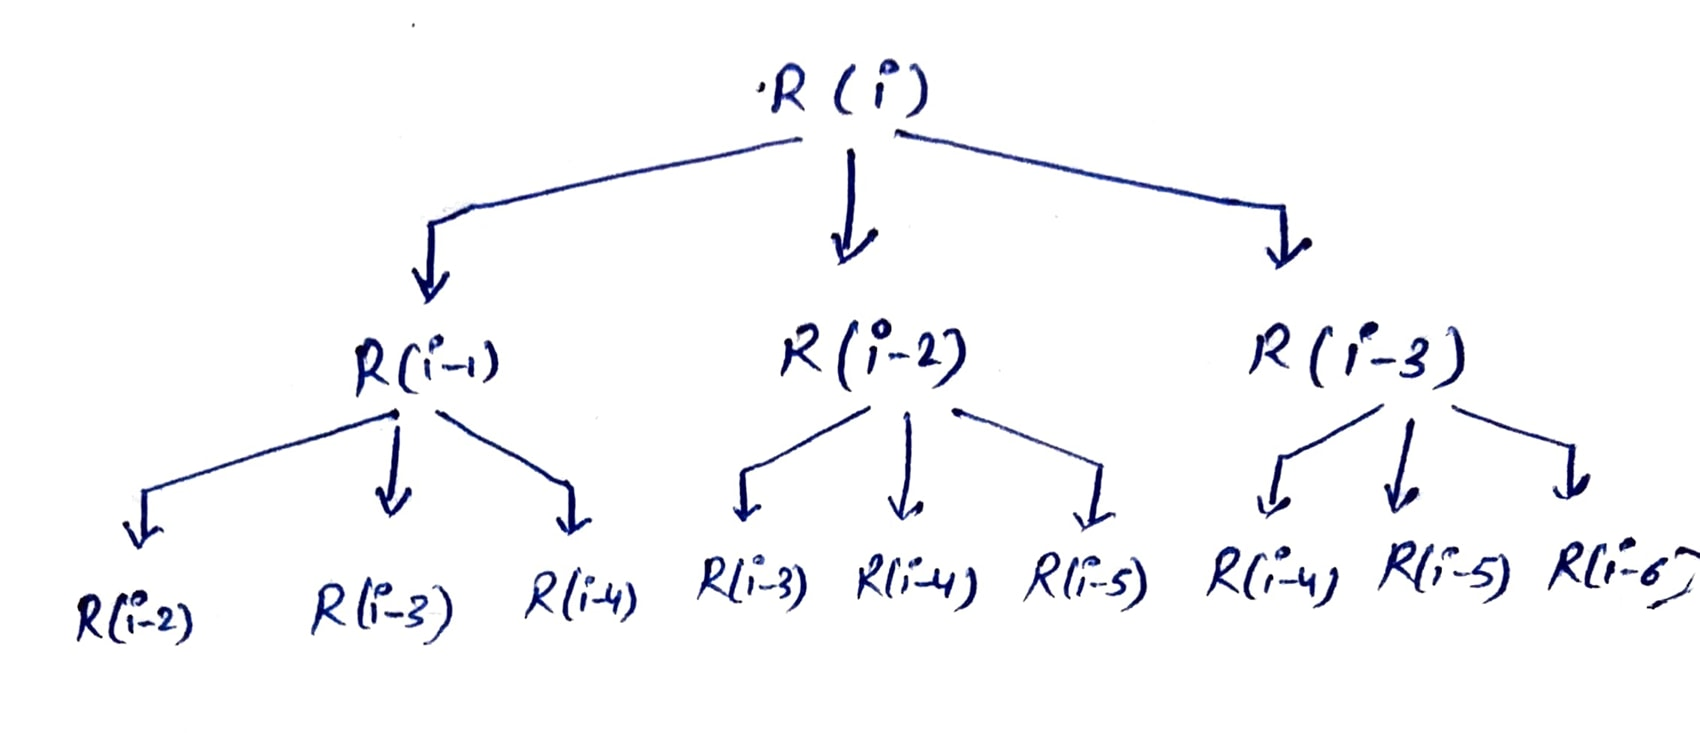
\includegraphics[scale=0.2, angle=-1]{recursionTree.jpeg}


\end{enumerate}

\newproblem
\textbf{Big Oh Definitions}

\underline{Definition 1}:
It says that, after a certain point $(n=n_0)$, $f(n) < g(n)$.
As Big-Oh gives the strict upper bound, then $g(n) \geq f(n)$ and this is possible iff $c_1$ is a positive constant i.e. $c_1>0$ and provided that $n_0$ cannot be a negative value.\\
So, if $f(n) \leq c_1 \cdot g(n)$ where $c_1>0$, then $f(n)=O_1(g(n))$ where $n>n_0$ and $n_0>0$.

\underline{Definition 2}:
It says that, all the Big-Oh conditions should be satisfied i.e. $n_0>0$ and $c_2$ should be positive value i.e. $c_2>0$.\\
So, if $f(n) \leq c_2 \cdot g(n)$ where $c_2>0$, then $f(n)=O_2(g(n))$ where $n>n_0$ and $n_0>0$.

From above, $f(n) = O_1(g(n)) = O_2(g(n))$ for all $g$.

\end{document} 
